\setlength{\columnsep}{3pt}
\begin{flushleft}

\begin{itemize}
	\item \textbf{ISO} stands for \textbf{International Organization of Standardization}.
	\item ISO is model for \textbf{Open System Interconnection (OSI)}.
	\item The ISO-OSI model is a \textbf{seven} layer architecture.
	\item It defines seven layers or levels in a \textbf{complete communication system}.
\end{itemize}

\begin{figure}[h!]
	\centering
	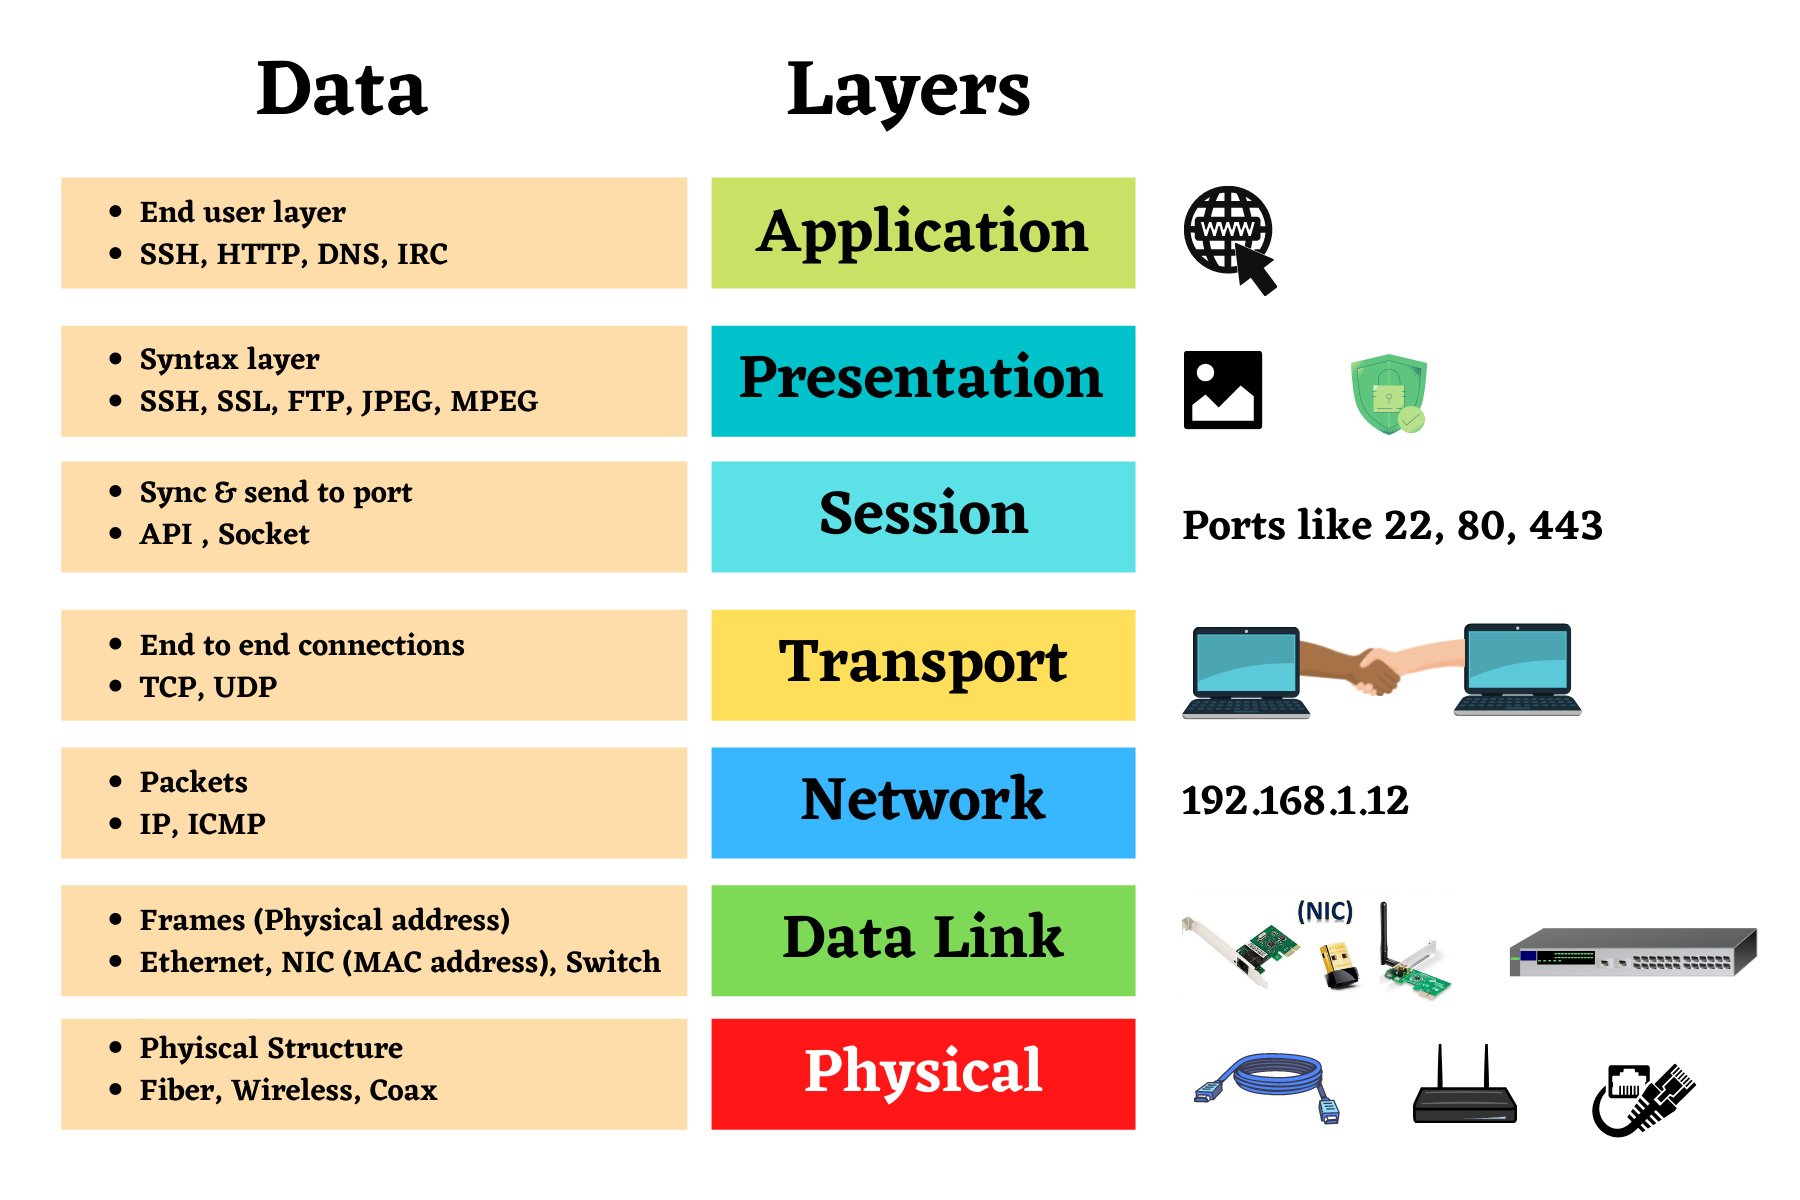
\includegraphics[scale=0.3]{content/chapter14/images/iso-osi.png}
	\caption{ISO OSI model}
	\label{fig:iso_osi}
\end{figure}

Let's see IP address in detail.

	
	
\end{flushleft}
\newpage


